%%%%%%%%%%%%%%%%%%%%%%%%%%%%%%%%%%%%%%%%%
% University/School Laboratory Report
% LaTeX Template
% Version 3.1 (25/3/14)
%
% This template has been downloaded from:
% http://www.LaTeXTemplates.com
%
% Original author:
% Linux and Unix Users Group at Virginia Tech Wiki 
% (https://vtluug.org/wiki/Example_LaTeX_chem_lab_report)
%
% License:
% CC BY-NC-SA 3.0 (http://creativecommons.org/licenses/by-nc-sa/3.0/)
%
%%%%%%%%%%%%%%%%%%%%%%%%%%%%%%%%%%%%%%%%%

%----------------------------------------------------------------------------------------
%	PACKAGES AND DOCUMENT CONFIGURATIONS
%----------------------------------------------------------------------------------------

\documentclass{article}

%\usepackage[version=3]{mhchem} % Package for chemical equation typesetting
%\usepackage{siunitx} % Provides the \SI{}{} and \si{} command for typesetting SI units
\usepackage{graphicx} % Required for the inclusion of images
%\usepackage{natbib} % Required to change bibliography style to APA
\usepackage{amsmath} % Required for some math elements 
\usepackage{float}
\usepackage{changepage}



\setlength\parindent{0pt} % Removes all indentation from paragraphs

%\renewcommand{\labelenumi}{\alph{enumi}.} % Make numbering in the enumerate environment by letter rather than number (e.g. section 6)

%\usepackage{times} % Uncomment to use the Times New Roman font

%----------------------------------------------------------------------------------------
%	DOCUMENT INFORMATION
%----------------------------------------------------------------------------------------

\title{Fundaments of HPC \\ Second Assignment} % Title

\author{Nicola \textsc{Domenis}} % Author name

\date{\today} % Date for the report

\begin{document}

\maketitle % Insert the title, author and date

\begin{center}
\begin{tabular}{l r}

\end{tabular}
\end{center}

% If you wish to include an abstract, uncomment the lines below
% \begin{abstract}
% Abstract text
% \end{abstract}

%----------------------------------------------------------------------------------------
%	SECTION 1
%----------------------------------------------------------------------------------------

\section{Introduction}

We present the second assignment in the course of FHPC. We will discuss about:


% If you have more than one objective, uncomment the below:
\begin{description}
\item[Exercise Zero] \hfill \\
Objective 1 text
\item[Exercise One] \hfill \\
Objective 2 text
\end{description} 
 
%----------------------------------------------------------------------------------------
%	SECTION 2
%----------------------------------------------------------------------------------------

\section{Exercise zero}

We start by observing two slightly different codes: 01\_array\_sum.c
and 04\_touch\_by\_all.c . They implement the same algorithm: summing the first N natural integers. They both use the OpenMP standard to take on a parallel approach with multiple threads.
The analysis of the programs can start by a strong scalability test.
We report the elapsed times versus the number of cores and also the speedups versus the number of cores:

\begin{figure}[H] % [h] forces the figure to be output where it is defined in the code (it suppresses floating)
	\centering
	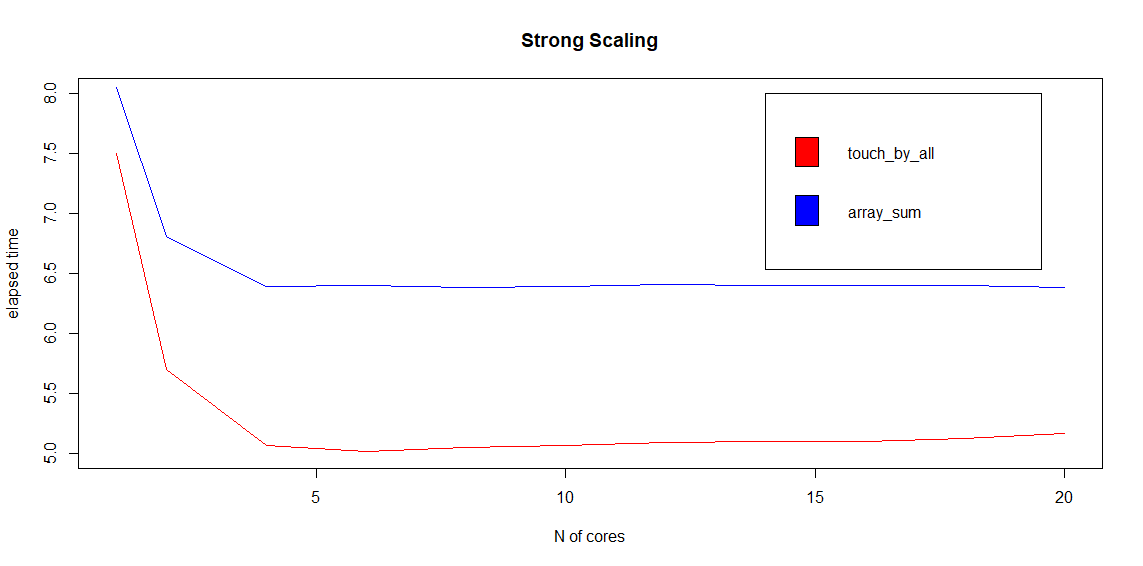
\includegraphics[width=0.8\columnwidth]{graphs/exercise_0_strongscaling} % Example image
	\caption{Elapsed times for $N=10^9$}
\end{figure}

\begin{figure}[H] % [h] forces the figure to be output where it is defined in the code (it suppresses floating)
	\centering
	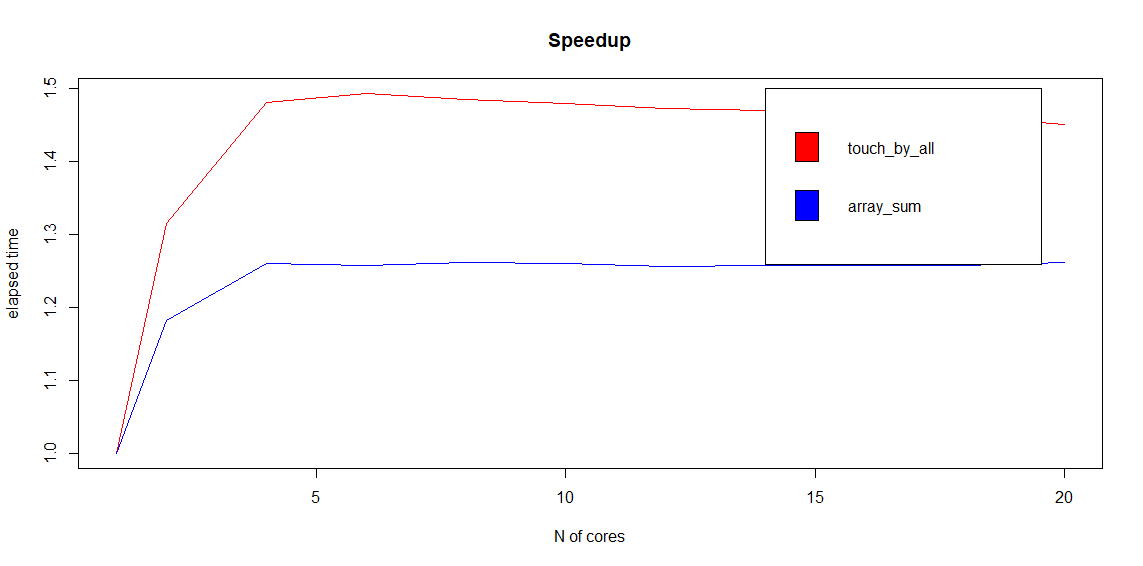
\includegraphics[width=0.8\columnwidth]{graphs/exercise_0_speedup} % Example image
	\caption{Speedup for $N=10^9$}
\end{figure}


We see that the code scales for the same size of the problem and that the code that implements the "`touch by all"' policy is faster.

Then we can see how to calculate the parallel overhead. We can use the formula $ e(n,p) =\frac{\frac{1}{S_p(n,t)}-\frac{1}{p}}{1-\frac{1}{p}}$ to estimate the parallel overhead. A plot with the measures we have would return:

\begin{figure}[H] % [h] forces the figure to be output where it is defined in the code (it suppresses floating)
	\centering
	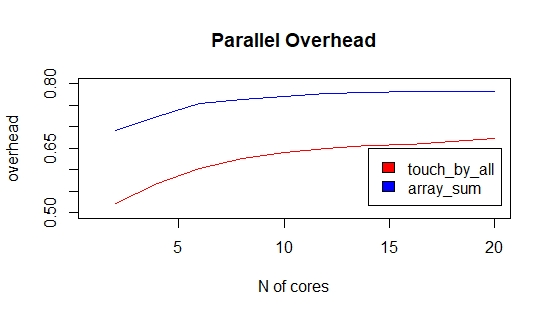
\includegraphics[width=0.8\columnwidth]{graphs/exercise_0_overhead} % Example image
	\caption{Overhead for $N=10^9$}
\end{figure}
The touch\_by\_all code once again is better than the array\_sum code, since it has a lower parallel overhead.
But both lines are growing, showing that both codes have a serious parallel overhead problem.

Now lets compare some valuable metrics for the two codes' executions:

\begin{adjustwidth}{-3cm}{}
\begin{tabular}[H]{l|l |l l l l| l l}
Metric & measures&&&&&mean&\\
CPU cycles& array\_sum &372889698& 143797361&671828181&373809554&390581199&-\\
          & touch\_by\_all&602487792&16412868&15030736&15901403&162458200&= \\
&&&&&&&	228122999\\				
					\hline
Cache misses & array\_sum&9459& 11492&49514&9484&19987.25&-\\
          & touch\_by\_all& 10356&10256 & 8417&12081&10277.5&=\\
&&&&&&&	 9709.75\\				
\hline
Elapsed time   & array\_sum& 0,014486573&0,007287606&0,024476034& 0,014344770&0.01514875&- \\
          & touch\_by\_all &0,021872540&0,002893806&0,002676134&0,002677902&0.007530096&=\\
					&&&&&&&	 0.00761865\\				
\hline
\end{tabular}
\end{adjustwidth}
Even if the single performances, measured with Perf, are quite similar in their randomness, we see that the touch\_by\_all code outperforms in average the array\_sum code in all the metrics.
%----------------------------------------------------------------------------------------
%	SECTION 3
%----------------------------------------------------------------------------------------

\section{Exercise 1}

We need to rewrite the code mpi\_pi.c by means of OpenMP directives. We had to solve all the problems we encountered in lesson, like avoiding race conditions and false sharing.
In the end we produced the simple code openmp\_pi.c.
We show the plots for the strong and weak scalability:


\begin{figure}[H] % [h] forces the figure to be output where it is defined in the code (it suppresses floating)
	\centering
	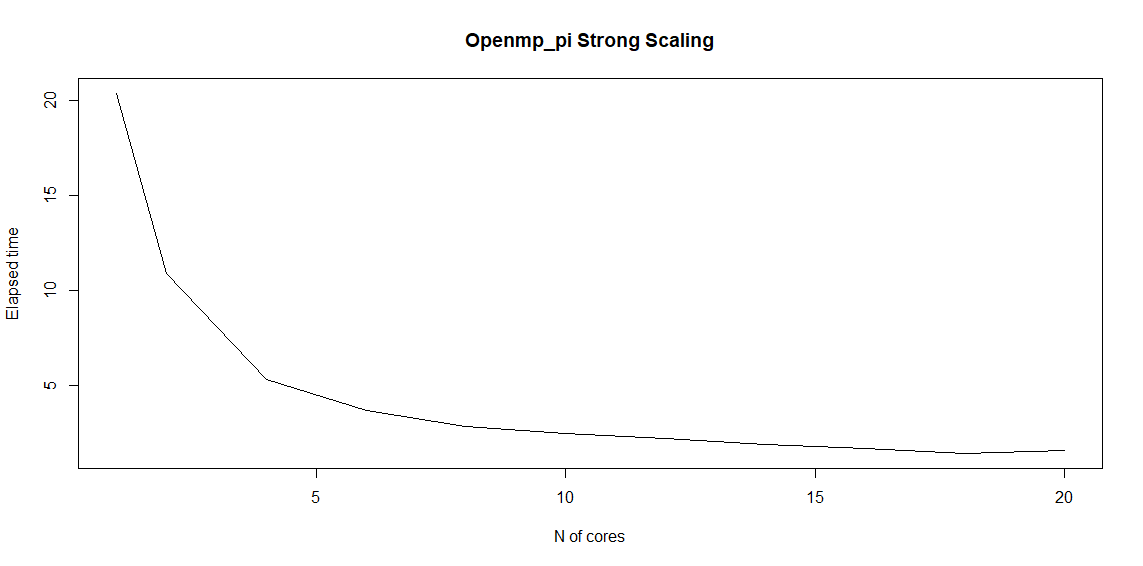
\includegraphics[width=0.8\columnwidth]{graphs/openmp_pi_strongscaling} % Example image
	\caption{Speedup for $N=10^9$}
\end{figure}
\begin{figure}[H] % [h] forces the figure to be output where it is defined in the code (it suppresses floating)
	\centering
	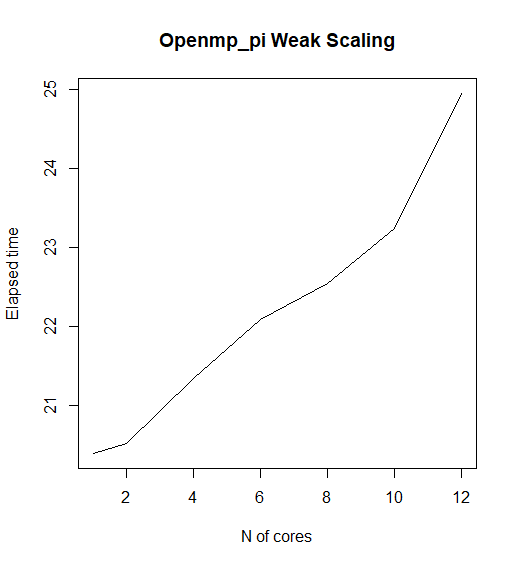
\includegraphics[width=0.8\columnwidth]{graphs/openmp_pi_weakscaling} % Example image
	\caption{Speedup for $N=10^4*P$}
\end{figure}

The code scales very well, the speedup is almost linear. But the weak scalability doesn't hold.
%----------------------------------------------------------------------------------------
%	SECTION 4
%----------------------------------------------------------------------------------------

\section{Results and Conclusions}

The atomic weight of magnesium is concluded to be , as determined by the stoichiometry of its chemical combination with oxygen. This result is in agreement with the accepted value.

\begin{figure}[h]
\begin{center}
%\includegraphics[width=0.65\textwidth]{placeholder} % Include the image placeholder.png
\caption{Figure caption.}
\end{center}
\end{figure}

%----------------------------------------------------------------------------------------
%	SECTION 5
%----------------------------------------------------------------------------------------

\section{}


The most obvious source of experimental uncertainty is the limited precision of the balance. Other potential sources of experimental uncertainty are: the reaction might not be complete; if not enough time was allowed for total oxidation, less than complete oxidation of the magnesium might have, in part, reacted with nitrogen in the air (incorrect reaction); the magnesium oxide might have absorbed water from the air, and thus weigh ``too much." Because the result obtained is close to the accepted value it is possible that some of these experimental uncertainties have fortuitously cancelled one another.

%----------------------------------------------------------------------------------------
%	SECTION 6
%----------------------------------------------------------------------------------------

\section{Answers to Definitions}

\begin{enumerate}
\begin{item}
The \emph{atomic weight of an element} is the relative weight of one of its atoms compared to C-12 with a weight of 12.0000000$\ldots$, hydrogen with a weight of 1.008, to oxygen with a weight of 16.00. Atomic weight is also the average weight of all the atoms of that element as they occur in nature.
\end{item}
\begin{item}
The \emph{units of atomic weight} are two-fold, with an identical numerical value. They are g/mole of atoms (or just g/mol) or amu/atom.
\end{item}
\begin{item}
\emph{Percentage discrepancy} between an accepted (literature) value and an experimental value is
\begin{equation*}
\frac{\mathrm{experimental\;result} - \mathrm{accepted\;result}}{\mathrm{accepted\;result}}
\end{equation*}
\end{item}
\end{enumerate}

%----------------------------------------------------------------------------------------
%	BIBLIOGRAPHY
%----------------------------------------------------------------------------------------
%---------------------------------------------------------------------------------------


\end{document}